\chapter{Concept \label{cha:concept}}
Establishing a connection between the latest advances in NLP and anomaly detection in system log data is a recently emerged field in research. The need for using language models to convert log events into word embeddings emerges from the weaknesses of older anomaly detection approaches that are not flexible enough to cope with the complex nature of system log data. There exist difficulties in reusing previously obtained knowledge from training on data from a given dataset and transferring it to a differently structured dataset. Most proposed techniques for solving the problem of anomaly detection in system log data suffer from not being transferable and being non-resilient to changing log data. The objective of this work is to provide a means to automatically detect anomalies in logs that are potentially affected by processing noise and changes of log events by updates of the underlying software, and to transfer knowledge obtained from a dataset of log sequences to another dataset of logs with a transfer method.

In section \ref{sec:problem_statement}, the general problem statement is given, and necessary requirements for this work are specified. 
In the following section \ref{sec:overall_system}, the overall system architecture with its components is outlined and visualised.
In section \ref{sec:learning} the developed approaches, including the baseline approach, are explained in detail. There exist three approaches, (1) the baseline approach featuring learning of sentence level log line representations with the help of an auto encoder on the basis of word level language representations and classification using regression, followed by the (2) regression and (3) multi-class classification approach using log line representations obtained by a language model which is able to transform log lines on sentence level.
In section \ref{sec:transferlearning} the transfer learning mechanism is described in detail.
In the final section \ref{sec:improvements} possible improvements of the proposed approach are presented.


\section{Problem Statement and Prerequisites \label{sec:problem_statement}}
Logs are print statements inside programs which are defined by a fixed sequence of code statements written by developers. The execution of a program is defined by these statements, and therefore follows a predetermined pattern. Hence, the produced logs must also follow certain patterns, chronological orders, and proportional relationships between number of occurrences of logs with each other. These logs must be first brought into an appropriate form, in .
%TODO

\subsection{Formal problem definition \label{sec:formal_problem_definition}}
A log is a sequence of ASCII characters, which is denoted by the set $\mathcal{A}$ that form unstructured messages $M = (m_0, m_1, ..., m_n)$ with every character of $m_i \in \mathcal{A}$. Log messages consist of tokens - most tokens are English words, but do also include special characters. The number of tokens from which a log message can consist of, varies. 
Let $g: \mathcal{A}^i \rightarrow \mathbb{R}^w$ be a function that takes a variable length of $i$ tokens that make up a log message and maps them to a fixed length vector of dimension $w$. This is the function which represents the computation of embeddings. $E = (e_0, e_1, ..., e_n)$ is the sequence of vectors based on $M$, parsed and transformed into embedding representations. Let $\mathcal{B} = (b_0, b_1, ..., b_n)$ be the dataset where every $b_i \in {0,1}$ denotes if the log event represented by $e_i$ is anomalous $(1)$ or not $(0)$. $\hat{b_i}$ denotes the system's prediction for $b_i$.

\textit{Multi-classification}: For every distinct log template, we assign $C = \{c_0, c_1, ..., c_k\}$ to be the set of distinct class keys. Let $g: \left|s\right| \times \mathbb{R}^w \rightarrow \mathbb{N},\;  g(E_i, \Psi) = \mathbb{R}^k$ be a function computed by a neural network, that given a subsequence of $s$ vectors out of the dataset $E$, namely $E_i = (e_i, ..., e_{i+s})$, returns a probability distribution $Pr_i[e_{i+s+1}|E_i]$ = $(c_0: p_0, c_1: p_1, ..., c_k: p_k)$, describing the probability for each template class from $C$ to appear as the next class at index $i+s+1$, given $E_i$. The objective is to learn the parameters $\Psi$, so that for each fixed length sequence of vectors, the function predicts the correct subsequent class. If one of the top $q$ candidate classes matches the actual class, then $\hat{b_i} = 0$ is returned, if it does not match the actual class, $\hat{b_i} = 1$ is returned.

\textit{Regression}: Let $h: \left|s\right| \times \mathbb{R}^w \rightarrow \mathbb{R}^w, \; h(e_i, s, \Phi)=d$ be a function computed by a neural network, that based on a sequence of $s$ vectors $E = (e_j, ..., e_{j+s})$ predicts the vector $d$ at index $j+s+1$. The objective in this case is to learn parameters $\Phi$, so that the system predicts the vector following the sequence of vectors of length $s$. If the distance between the predicted vector $d$ and the actual vector $e_{j+s+1}$ is above or below certain threshold values, which will be computed by the q-th percentile of all loss values from the original dataset, then $\hat{b_i} = 1$ is returned, if it is inside these thresholds, then $\hat{b_i} = 0$ is returned.

\subsection{Requirements and Assumptions \label{sec:requirements_and_assumptions}}
\begin{enumerate}
	\item The model requires a word vectors by a language model that has been pre-trained on a sufficiently large corpus.
	\item The model requires \textit{normal} log data, which does not contain anomalies for training.
	\item The model is not able to detect anomalies which are only in the variable part of the log messages. The model only considers the templates, i.e. keys.
\end{enumerate}



\section{System Overview \label{sec:overall_system}}
In this section, a broad overview of the overall system is presented, with figure \ref{fig:overall_system} illustrating the steps necessary for the learning procedure, followed by anomaly classification. 
The core concept can be outlined as follows: first, original log sequences are prepared, then a log parser is used to extract templates from the original log sequences and then transform the log sequences to template sequences. Afterwards, the template sequences are transformed into log sequence embeddings by a language representation model. This procedure is described in detail in section \ref{sec:pre_processing}. 

For the training part, the log sequence embeddings are fed into a LSTM, which learns to predict the next embedding, which is called the regression task, specified in section \ref{sec:regression} and coloured red in figure \ref{fig:overall_system} or the next sequence class, which is called the classification task, specified in \ref{sec:classification} and coloured blue in figure \ref{fig:overall_system}. The results of these predictions are then compared to the true subsequent log embedding or class of the true subsequent log template, in order to train the model to identify "normal" log data.

The prediction part involves two steps: first, the template sequences obtained from the original log sequences A are altered by changing the order of the sequences or manipulating the templates, as described in section \ref{sec:logs_alteration}. As a second step, these manipulated sequences are fed to the model which has been trained on embedding sequences not containing any alterations, thereby obtaining the model's predictions if a log line is anomalous or not.

Transfer learning builds onto this process. After a model has been trained as described on dataset A, pre-processing is conducted the same way on a new dataset B, thus obtaining template sequences and embedding sequences. For the classification task, the template sequences of dataset B are mapped to the class mappings of dataset A, and then used for prediction. The regression task functions analogously to learning without transfer. Transfer learning is described in detail in section \ref{sec:transferlearning}

\begin{figure}[H]
	\centering
	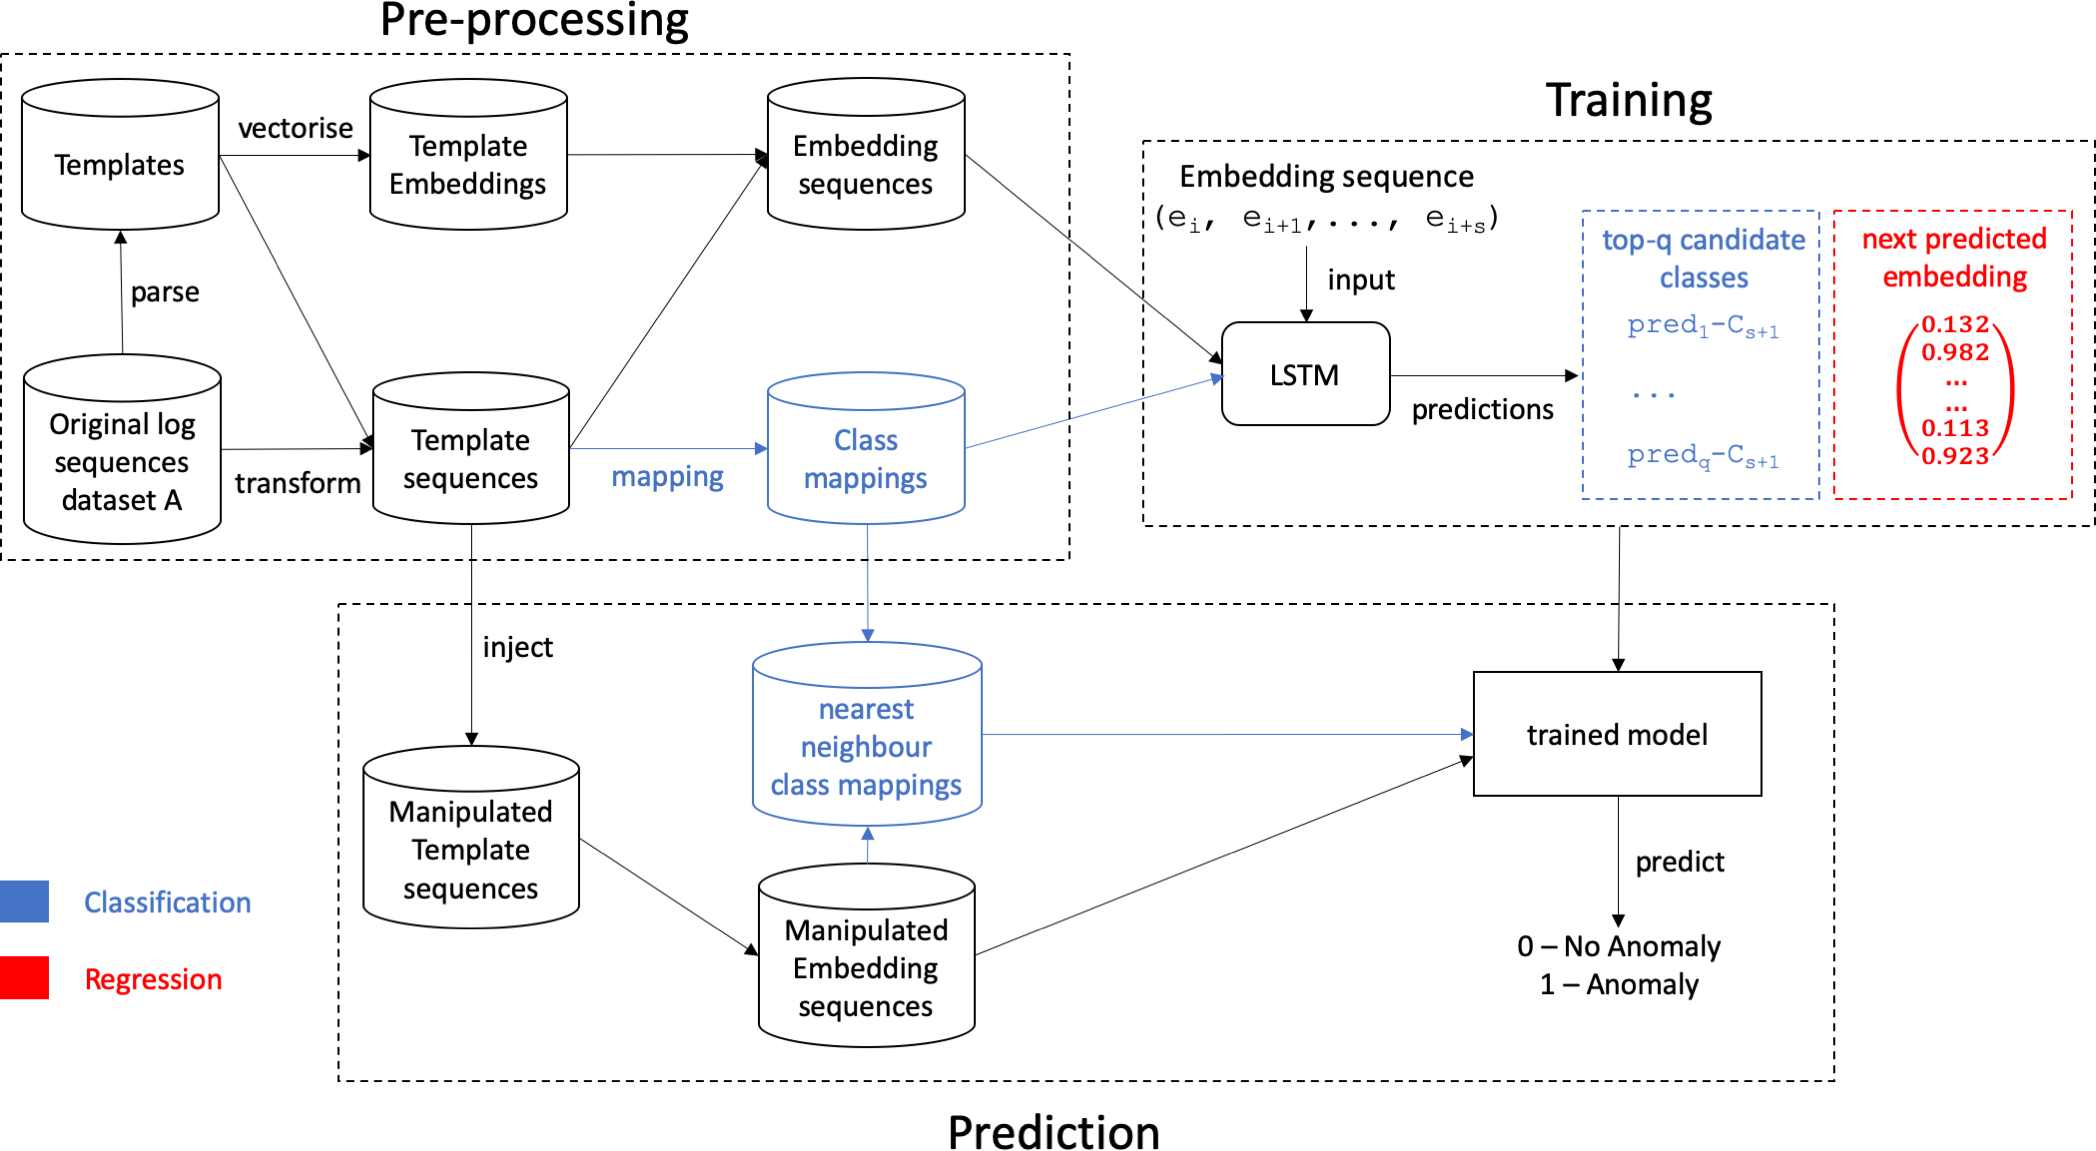
\includegraphics[width=15cm]{overall.png}
	\caption{Anomaly Detection System}
	\label{fig:overall_system}
\end{figure}

\section{Pre processing \label{sec:pre_processing}}
Log files are usually available in an unordered, raw state, and need to be ordered, parsed and transformed into an appropriate format so that they can be handled as sequences by a LSTM. The required steps for this purpose are outlined in this section. In the first subsection \ref{sec:conceptlogparsing}, the steps required for parsing logs are outlined, followed by the transformation into word embedding vectors in \ref{sec:word_vectorization}. A diagram illustrating the complete pre-processing pipeline can be see in figure \ref{fig:full_preprocessing_pipeline}

\subsection{Log Parsing}\label{sec:conceptlogparsing}
Log parsing is an important step for automated log analysis, as already described in section \ref{sec:backgroundlogparsing}, since raw log messages are unstructured data and contain a lot of extra information. The result of the execution of a log parser can be see in figure \ref{fig:parsing}. There are a few important aspects to note here: Not only does the log parsing step extract log templates, it also extracts other valuable information in a structured way, namely timestamps and, in this example the bulk id. Timestamps are needed, in order to make sure that the logs are in the correct chronological order, since it is possible, that system logs are an aggregation of log output of different sub-routines or different instances, which can happen concurrently, thus producing unordered logs. Additionally to sorting by timestamps, it can also be required to sort system logs by group ids, instance ids or bulk ids as in the example figure \ref{fig:parsing} in order to be able to observe each self-contained block separately from other blocks.

\subsection{Template cleansing \label{sec:template_cleansing}}
Even though log parsing and the aforementioned ordering steps largely improve the further processability of logs for sequential learning, by making it possible to single out the fundamental semantics of a log event, they are still partly made up of special characters and variable names. The following characters are removed:
\begin{enumerate}
	\item All non-character tokens such as delimiters, digits, and particularly variable placeholders (\verb!<*>!).
	\item All concatenations of words are split, for example \verb!sync_power_state! will be split into the separate words \verb!sync!, \verb!power! and \verb!state!
	\item All leading, trailing and repeated whitespace characters are removed.
\end{enumerate}

\subsection{Word vectorisation \label{sec:word_vectorization}}
After the aforementioned pre-processing steps, the log events are transformed into word embeddings, using a language model that is able to convert words or whole sentences into word or sentence embedding, effectively representing function $g$ defined in \ref{sec:formal_problem_definition}. Satisfying the following two requirements is essential in the context of providing suited word embeddings for the anomaly detection task:
\begin{itemize}
	\item Distinguishability: Word embeddings should capture the difference between log events with differing semantics. For example "\verb!<*> Terminating instance!" and "\verb!<*> Deleting instance files <*>!" are log events with highly different semantics, even though they contain equal (instance) and in the broader sense similar (terminating, deleting) words. This means their cosine distance should be high.
	\item Tolerance: Word embeddings should capture the similarity between different log events with same or very similar semantics. For example, the log event pair "\verb!<*>! \verb!Creating image!" is changed to "\verb!<*> Image created successfully!" or "\verb!VM up!" is changed to "\verb!VM started!". This in turn should result in a low cosine distance \cite{zhang2019robust}.
\end{itemize}

In order to compare the impact of the choice of a language model, two main approaches are implemented.

\subsubsection{Transformer-based Language Models \label{transformer-approach}}
In oder to be able to compare the quality different language model's word embeddings with regards to the task of anomaly detection, it is possible to easily swap the used language model for log event transformation. For this work, the pre-trained language models used for evaluation, are Bert, GPT-2 and XL-Transformers.



\subsection{Finetuning\label{sec:finetuning}}
Word embeddings models are usually provided pre-trained in different formats (e.g. with or without upper case), because training them from scratch is expensive - for Bert, it requires 4 days of training on 16 cloud TPUs for one language \cite{googlebert}. They are trained on large corpuses with unsupervised tasks. In order to make them more useful with regards to the task of anomaly detection, it is reasonable, to adjust the given pre-trained datasets using the log data corpora.

\subsection{Log Alteration\label{sec:logs_alteration}}
By altering log events, the evolution of log events is being simulated. Since software is changed by developers, also the log statements are subject to constant change. It is desirable to build a flexible model that does not have to be retrained after each update of a log producing software. Log alteration is also used to simulate a different dataset B based on a given dataset A, for applying transfer learning, as outlined in \ref{sec:transferlearning}.

Injection and alteration is done in a programmatically controllable manner. Various types of alterations are injected into original log data, either on the log event itself as in figure \ref{fig:changelogevent} or on the sequence of log events as in figure \ref{fig:changesequence}.

Three types of alterations are injected into the log events: a various amount of words is inserted between the tokens, for example words that appear in the context of logs, like "\textit{deleted}", "\textit{during}", "\textit{for}" or "\textit{time}", but for testing purposes, also words that are random in the context . Words can be also deleted. Finally, words can be replaced by new words. All of these alterations can be injected multiple times into the same log event. It is desirable that the system does not detect a log event as an anomaly, that has not been changed much, i.e. only one or two words have been added into a statement (e.g. if "\textit{* Took *.* seconds to deallocate network for instance.}" has been changed to "\textit{* Took \textcolor{red}{time} *.* seconds to deallocate network for \textcolor{red}{this} instance.}").
%TODO how many words threshold for anomaly detection

Additionally, it is possible to perform changes on the sequence of logs. In the following example, let $M = (m_i : i = 0, 1, 2, ..., n))$ be a sequence of log events:
\begin{itemize}
	\setlength\itemsep{-0.5em}
	\item events can be \textit{deleted} from the sequence, meaning that if the event at index $j$ is selected for deletion, the resulting sequence is $M_{del} = (m_0, ..., m_{j-1}, m_{j+1}, m_n)$.
	\item events can be \textit{shuffled}, meaning that if the event index $j$ is selected for shuffling at index $k$, the resulting sequence is $M_s = (m_0, ..., m_j, m_k, m_{k+1}, ..., m_{j-1}, m_{j+1}, ..., m_n)$
	\item events can be \textit{duplicated}, meaning that if the event at index $j$ is selected for duplication, the resulting sequence is $M_{dup} = (m_0, ..., m_j, m_j, m_{j+1}, ..., m_n)$
	\item new events can be \textit{inserted} meaning that if the event $m_{new}$ is inserted at index $j$, the resulting sequence is $M_{ins} = (m_0, ..., m_{new}, m_j, m_{j+1}, ..., m_n)$
	\item log sequences can be \textit{inverted}, the resulting sequence being $M_{inv} = (m_i : i = n, n-1, ..., 2, 1, 0)$
\end{itemize}

Just like for the insertion of alterations on the log events themselves, it is desirable of the system not to detect an anomaly for the deletion, duplication or shuffling of events, but for the insertion of anomalies into an event series, and the inversion of log events. These inserted anomaly events can be any type of log events that the system has not seen before.


\begin{figure}[H]
	\centering
	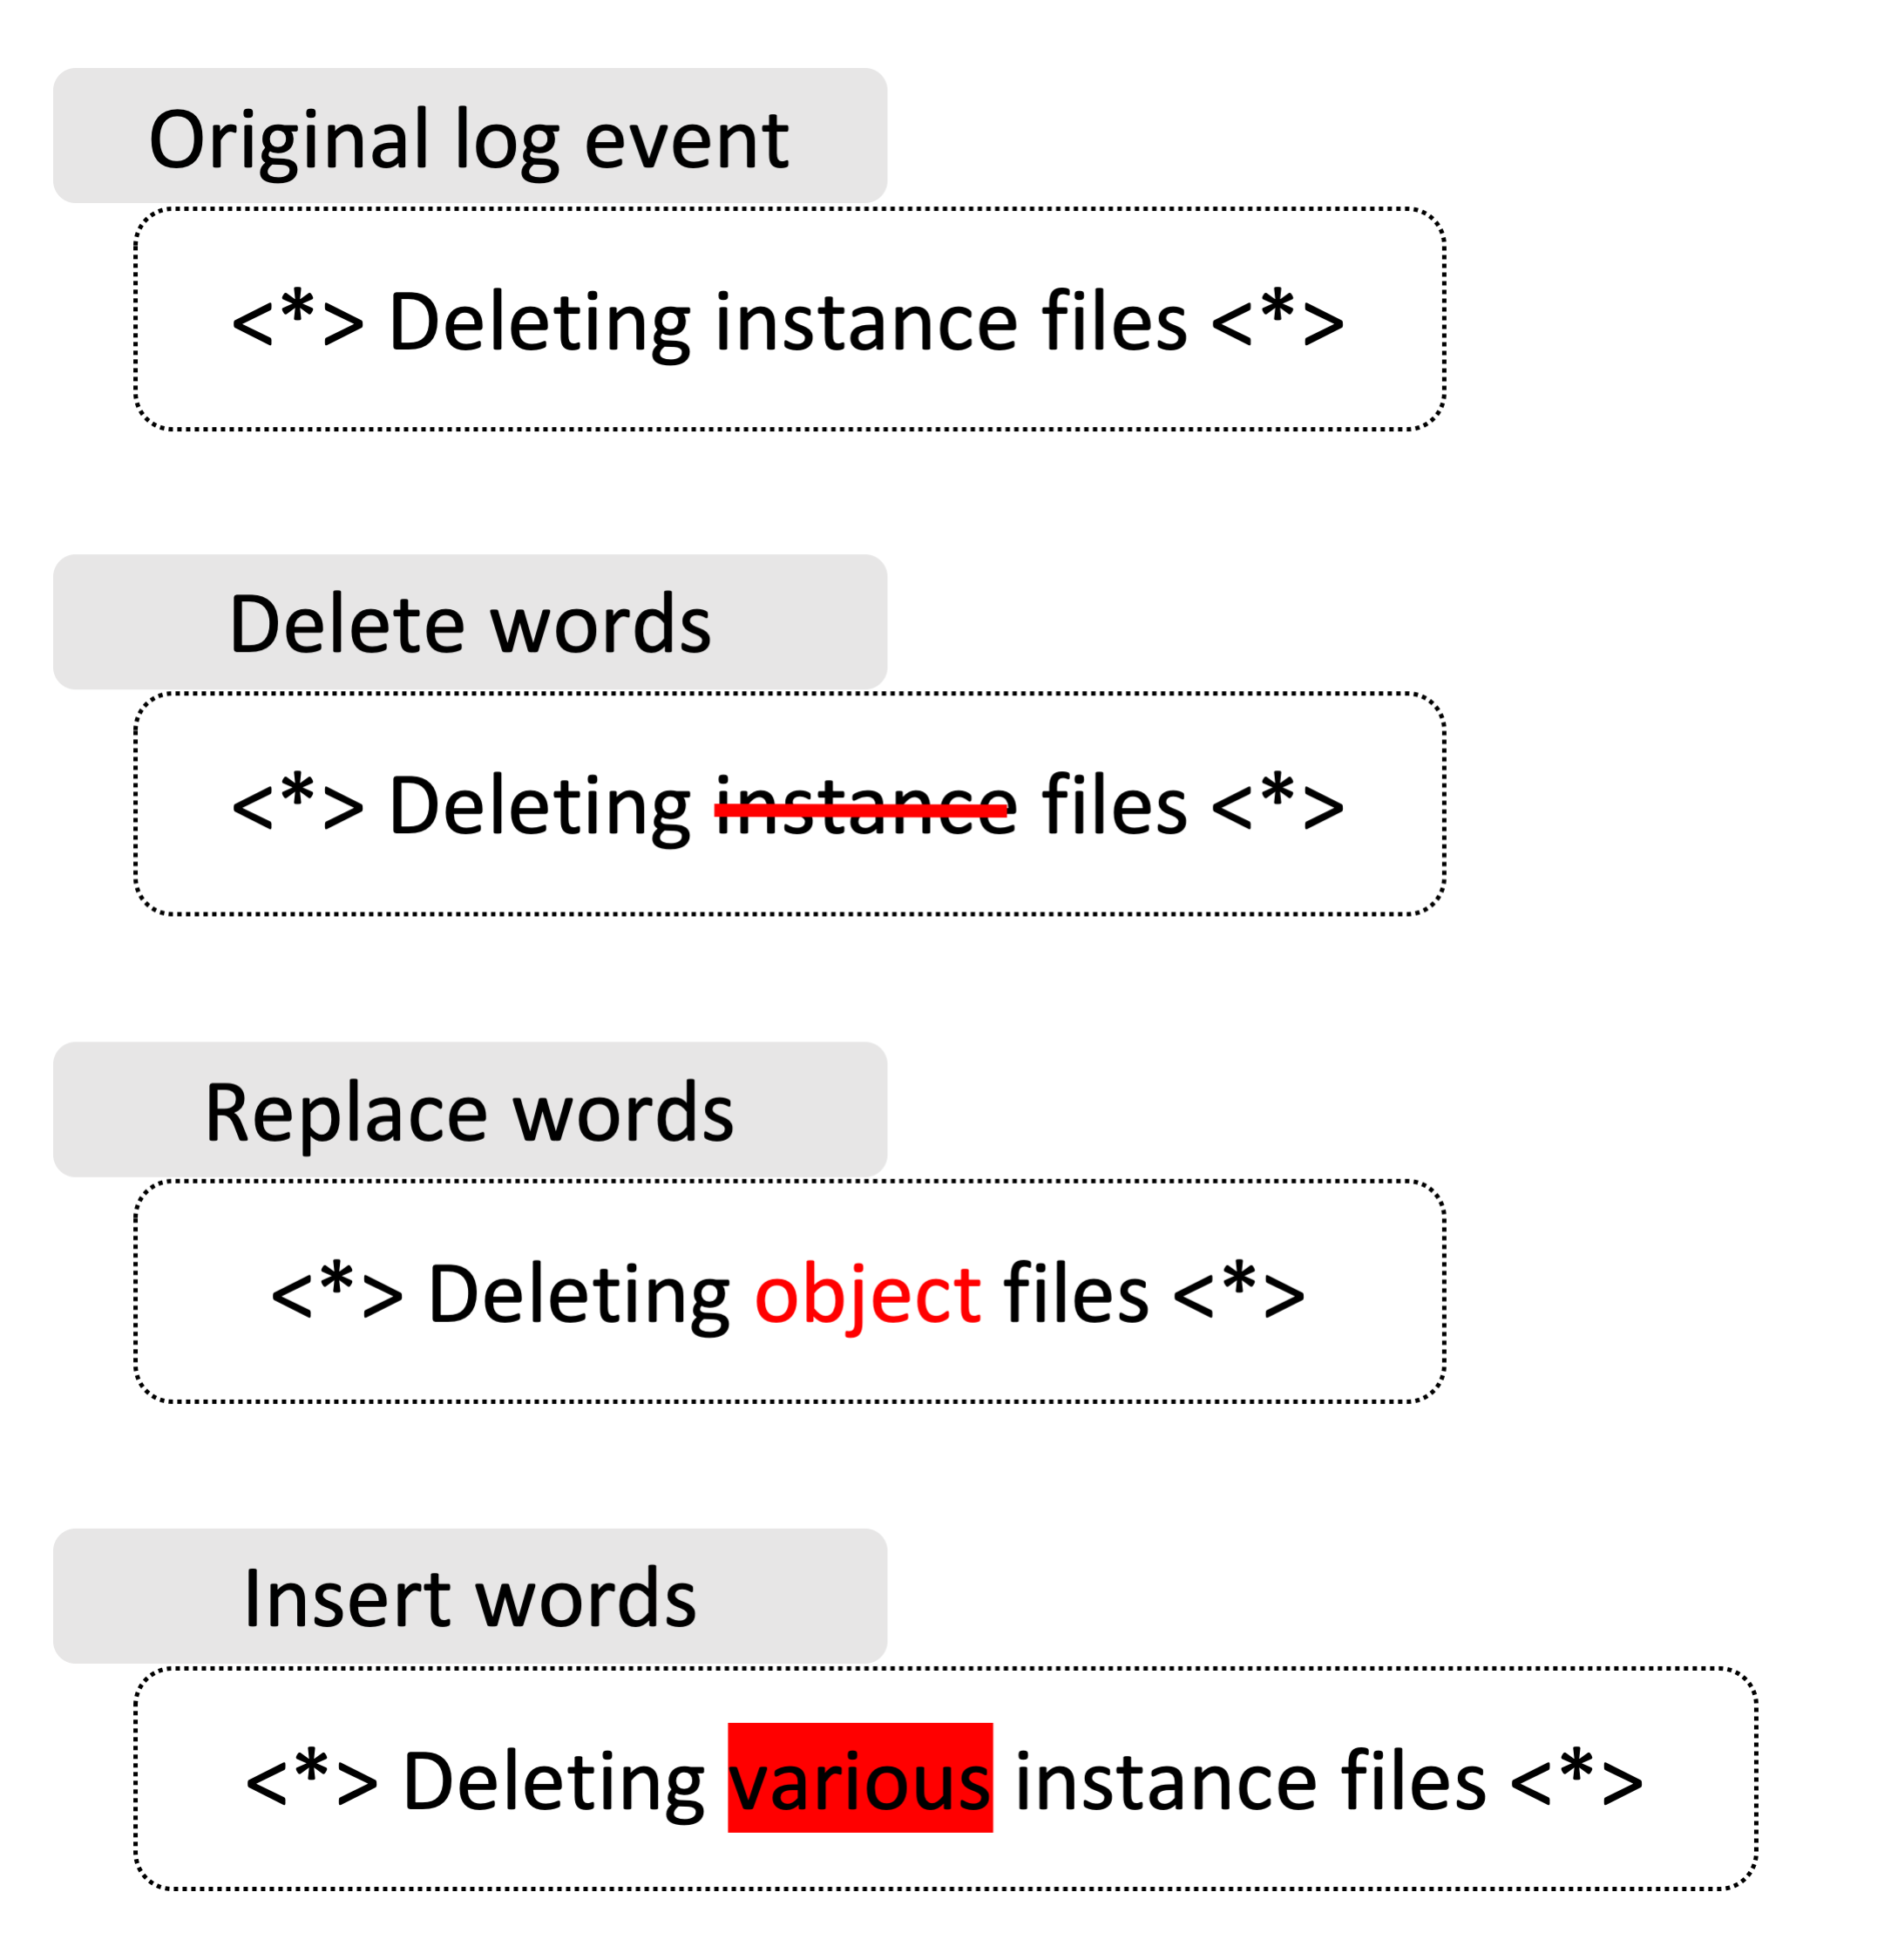
\includegraphics[width=6cm]{change_log_event.png}
	\caption{Altering log events.}
	\label{fig:changelogevent}
\end{figure}

\begin{figure}[H]
	\centering
	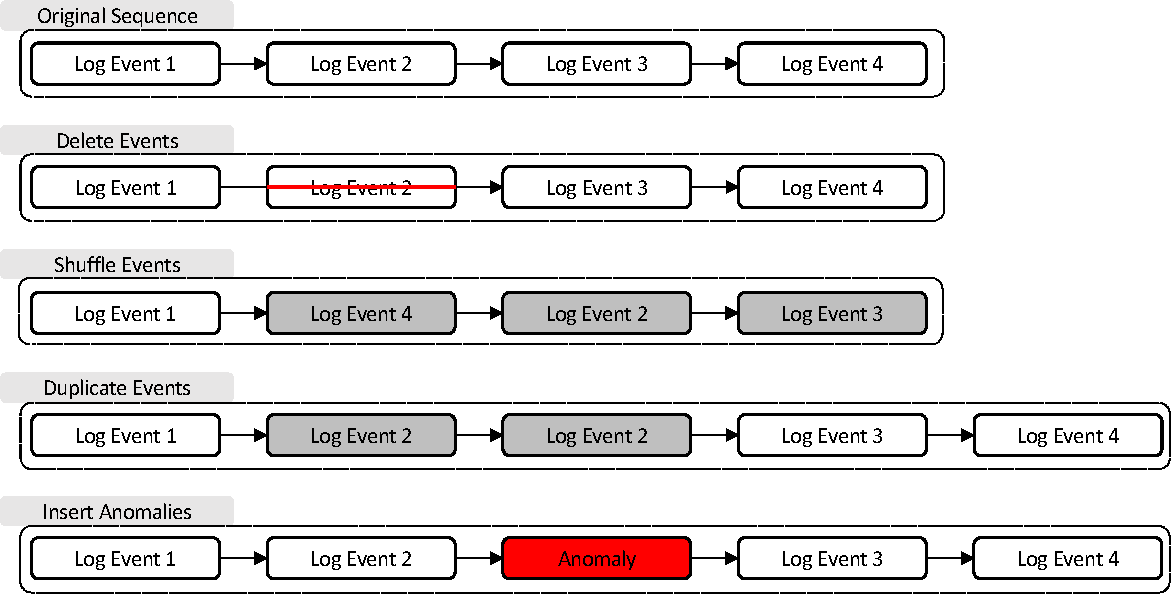
\includegraphics[width=13cm,height=15cm,keepaspectratio]{change_sequences.pdf}
	\caption{Altering log sequences.}
	\label{fig:changesequence}
\end{figure}




\section{Prediction Model\label{sec:prediction_model}}

\subsection{LSTM Model\label{sec:lstm-model}}
Through the aforementioned steps in \ref{sec:pre_processing}, all log events are transformed into word embeddings $e_i \in \mathbb{R}^w$. In order to learn sequences of logs, $s$ embeddings are concatenated to form an embedding sequence $E$. Taking a sequence of embeddings as input, a \textit{Bi-LSTM} neural network as described in \ref{sec:lstm} and \ref{sec:bi-lstm} is utilised to predict the class or embedding at position $s+1$. Figure \ref{fig:lstm_model} shows the structure of the Bi-LSTM. As a first step, a dropout is applied to the input sequence, which randomly drops out information in order to reduce overfitting and improve generalisation, before feeding it to the forward and backward layers of the Bi-LSTM. Then, the outputs of the Bi-LSTM are again fed into a dropout layer, followed by a fully connected layer, which reduces the output of the LSTM into the desired dimensions, i.e. $\mathbb{R}^w$ for regression and number of classes $c$ for multi-classification. Finally, an activation function $f$ is applied to the last output $o_{s_+1}$, log-softmax for multi-classification and linear for regression, respectively, in order to obtain the model's prediction $p_{s+1}$.


\begin{figure}[H]
	\centering	
	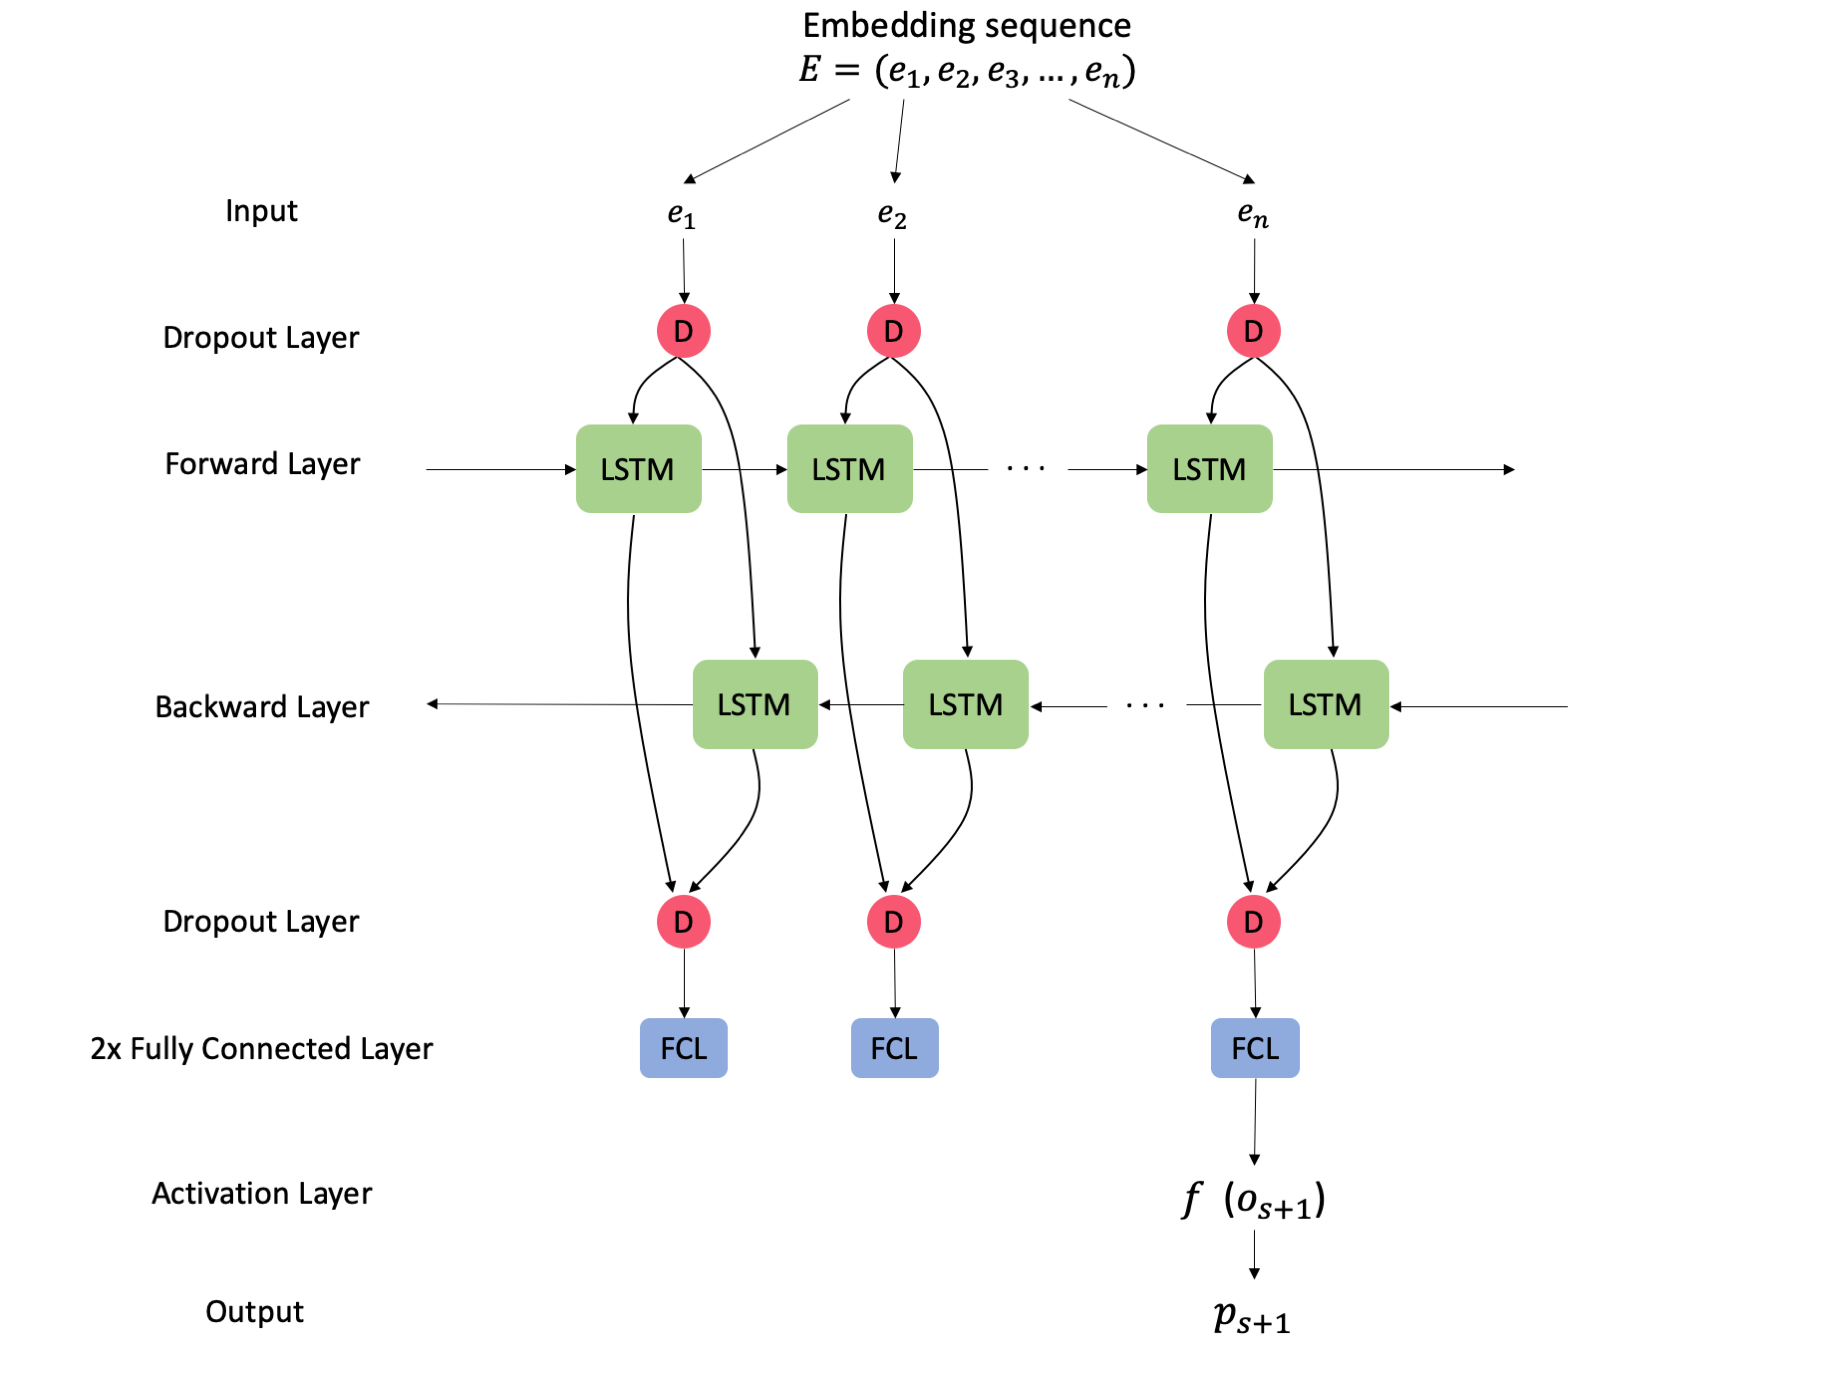
\includegraphics[width=16cm]{lstm_model.png}
	\caption{Bi-LSTM model}
	\label{fig:lstm_model}
\end{figure}

\subsection{Classification \label{sec:classification}}
For the multi-classification approach, the finite set of $n$ unique log event templates is mapped to class indices $(c \in \mathbb{N}^{+}: c \leq n)$. Training of the neural network is then performed on original log data that does not contain anomalies.
\begin{itemize}
\setlength\itemsep{-0.5em}
	\item The \textit{input} values of the training data have the dimensions $n$, $s$ and $w$, with $n$ being the number of unique log events, $s$ being the length of the sequence of word embeddings for which the neural network shall learn the consequent class and $w$ being the dimensionality of the log event embeddings.
	\item The \textit{target} values of the training data are structured as follows: for every sub-sequence of word embeddings $S_i = (i, ..., i+s)$, there is a corresponding class $c_{s+i+1}$ that stands for the template at position $s+i+1$. The system is trained to predict that class correctly.
\end{itemize}

After training has been executed on dataset A, the prediction phase starts, where a dataset B containing anomalies and alterations, as described in \ref{sec:logs_alteration}, can be processed by the neural network. For a new incoming dataset B, the system first has to match every template to the template classes of dataset A. For every template in dataset B, the nearest neighbour out of the templates of dataset A is determined and will get the respective class assigned, as depicted in figure \ref{fig:label_mapping}. This means in particular, that for every unique template, the corresponding word embedding is retrieved, and then every one of the word embeddings of dataset B is mapped to the word embedding from dataset A with the lowest cosine distance. Additionally, a threshold has to be found, so that if for a given word embedding in dataset B, no corresponding word embedding with a cosine distance below this threshold is found, that template shall not get a class assigned, this would otherwise lead to a situation where the log event \textit{"System restarted"} gets mapped to any of dataset A's template classes, which is not desirable behaviour.

After the matching process is finished, the system can read in the sequences of log events of dataset B. For every sequence of log events $S_i$ of length $s$, the system returns a probability distribution $Pr[c_{s+i+1}|S_i] = \{c_1 : p_1, c_2 : p_2, ..., c_n : p_n\}$ that denotes the probability of each log template class to appear as the consequent one. It is possible, that there are multiple candidates for the following template. For example, if the system is attempting to terminate an instance, then the corresponding template to class $c_{s+i+1}$ could be either '\textit{Instance terminated successfully}' or '\textit{Waiting for instance to terminate}'. The possible template classes $c_i$ are sorted based on their probabilities. A predicted template class is considered normal, if it is among the top $g$ candidates. It is marked as anomalous otherwise.
 

\begin{figure}[H]
	\centering
	\captionsetup{justification=centering}
	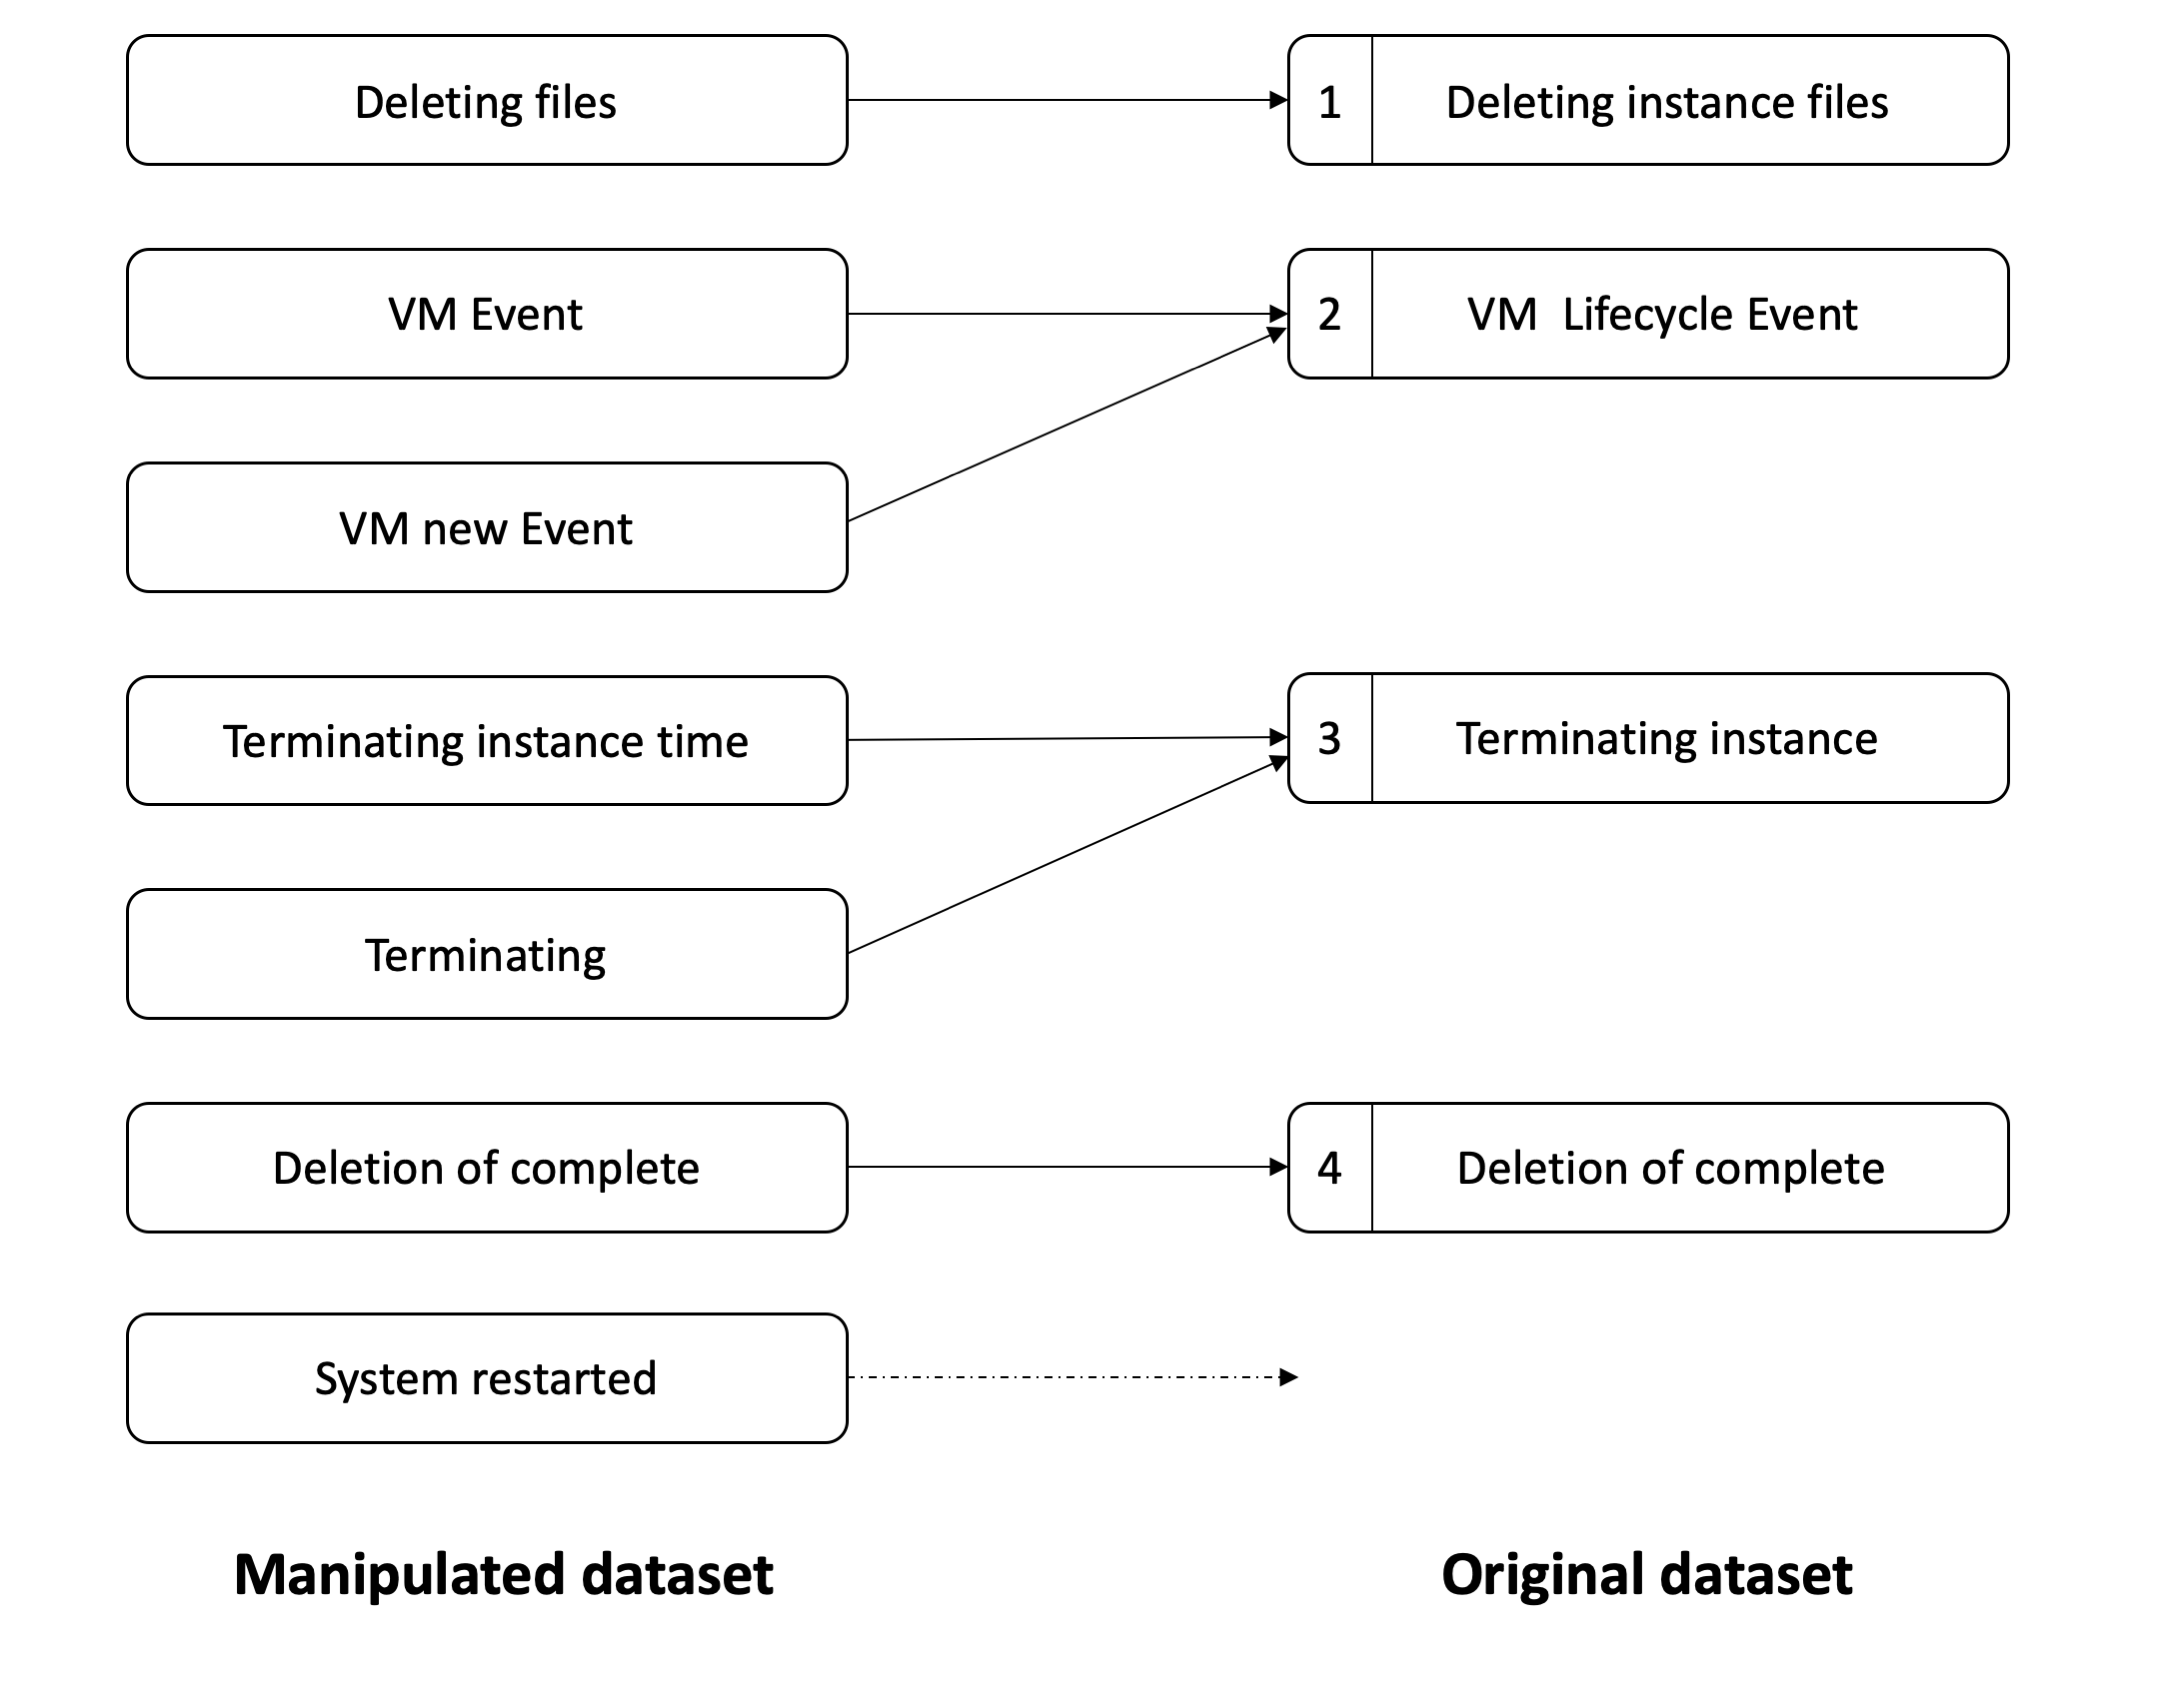
\includegraphics[width=12cm]{label_mapping.png}
	\caption{Template mapping}
	\label{fig:label_mapping}
\end{figure}

\begin{figure}[H]
	\centering	
	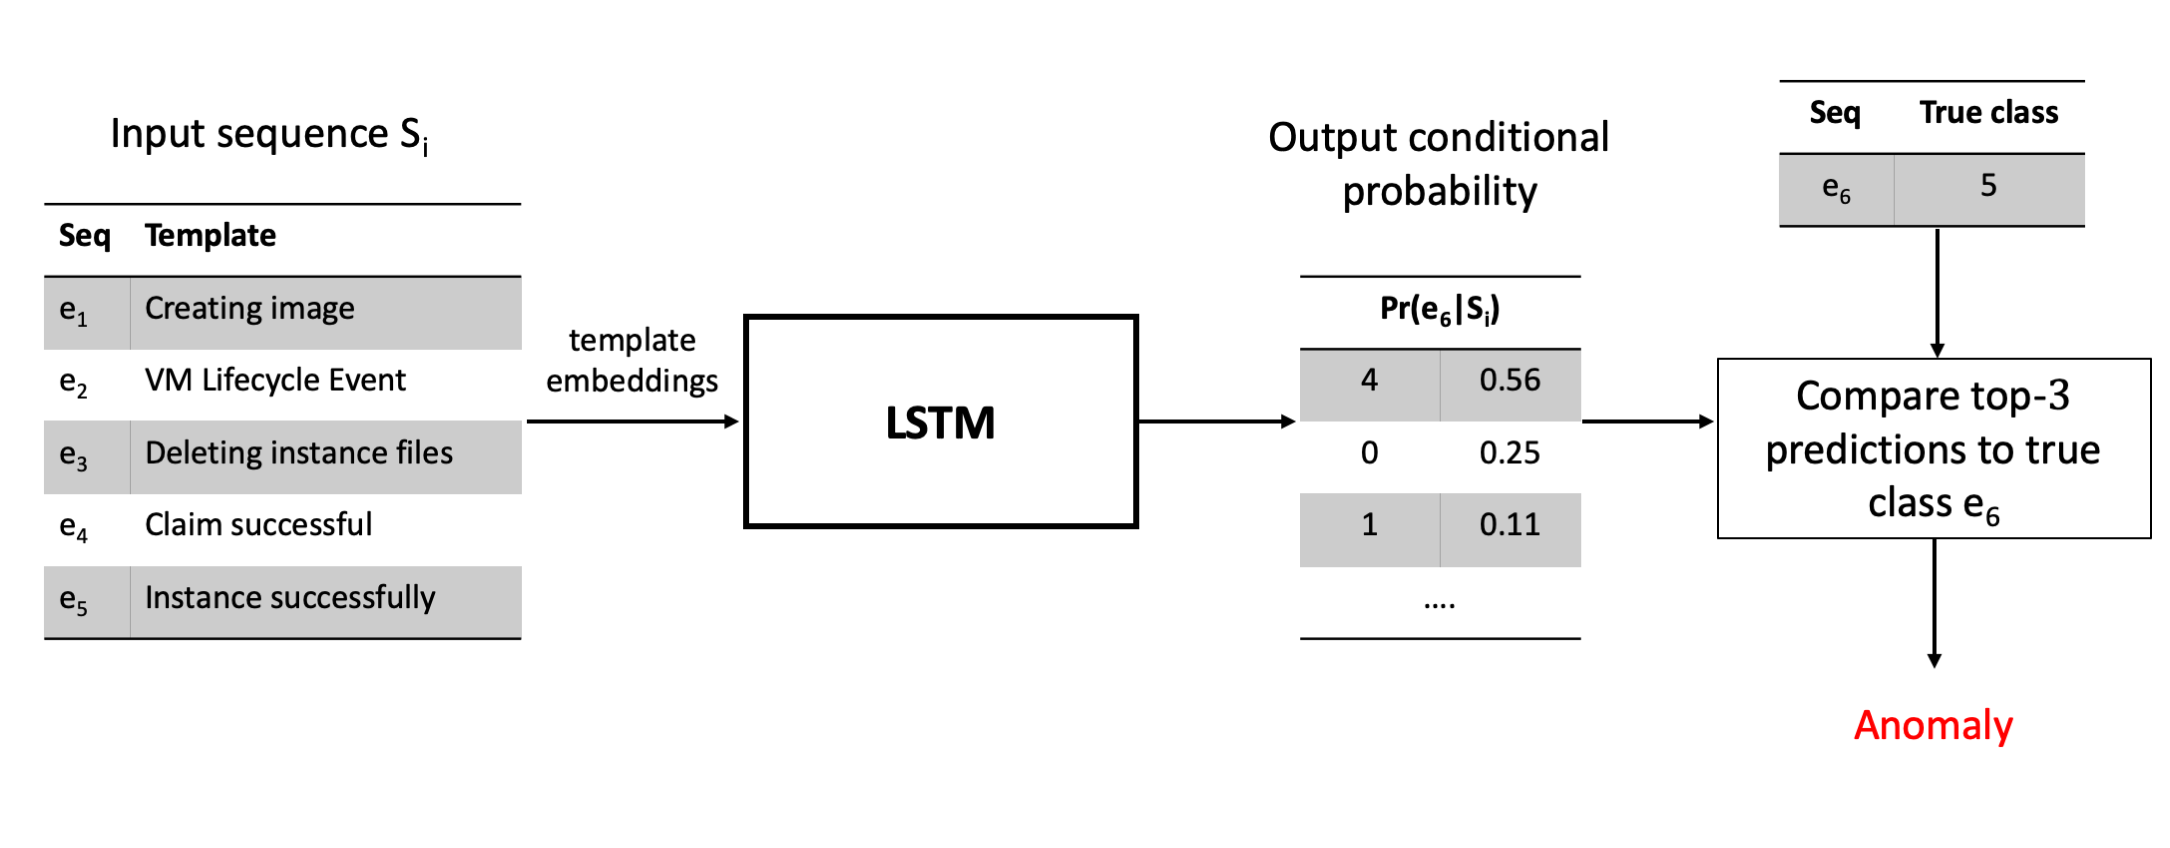
\includegraphics[width=15cm]{classification_detect.png}
	\caption{Class Prediction example for $g=3$}
	\label{fig:class_prediction}
\end{figure}

\subsection{Regression \label{sec:regression}}
For the regression approach, the neural network is trained to solve a regression task, with the input values of the training data being structured as described in \ref{sec:classification}, while the corresponding target value for the sequence of embeddings $E_i = (e_i, ..., e_{i+s})$ is the embedding of the log event at position $i+s+1$, meaning the neural network shall predict the next embedding $e_{i+s+1}$. After training on the original dataset, the mean squared error loss of every target word vector at position $i+s+1$ of the corresponding input sequence $E_i$, and the neural network's predicted word vector, is computed. Afterwards, the \textit{q-th} percentile of the agglomerated loss values of the original dataset is computed. The optimal value \textit{q} for the following purpose is to be determined by a simple grid-search. For the sequences of the manipulated test dataset, the loss values are computed in the same way as for the original dataset. The system will then mark every log event whose word embedding's loss value is above the calculated \textit{q-th} percentile as an anomaly (1), otherwise as non anomalous (0). This is depicted in figure \ref{fig:regression_with_threshold}.

\begin{figure}[htb]
  \centering
  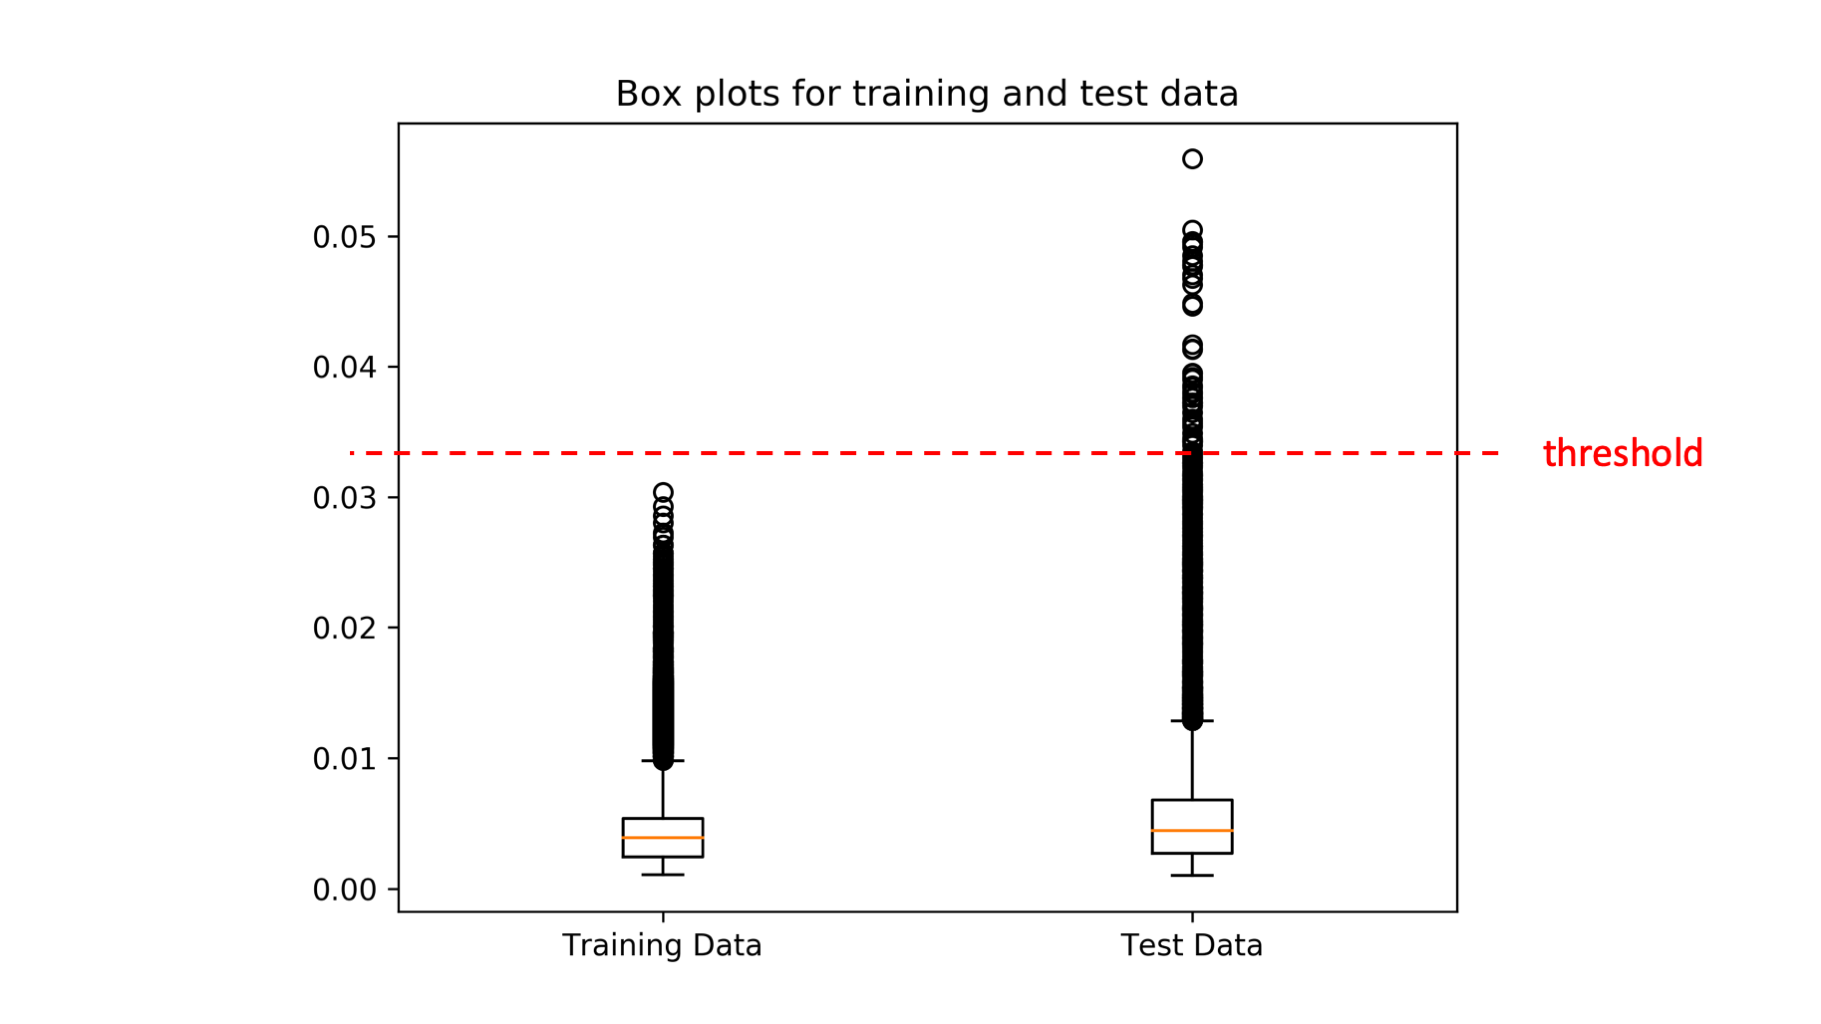
\includegraphics[width=15cm]{regression_box_plots_example.png} \\
  \caption{Box plots showing the distribution of loss values for training and test data.}
  \label{fig:regression_with_threshold}
\end{figure}


\section{Transfer Learning \label{sec:transferlearning}}
Transfer learning is the main focus of this work. It builds upon the aforementioned techniques and uses them to develop an infrastructure-agnostic anomaly detection model. With the help of these techniques, frequent re-training of models can be avoided and models trained on one dataset can be ported to be used with different datasets. The way transfer learning is executed differs from the classification approach, which is further outlined in \ref{sec:transfer_classification} and the regression approach, explained in \ref{sec:transfer_regression}. 

\begin{figure}[H]
	\centering
	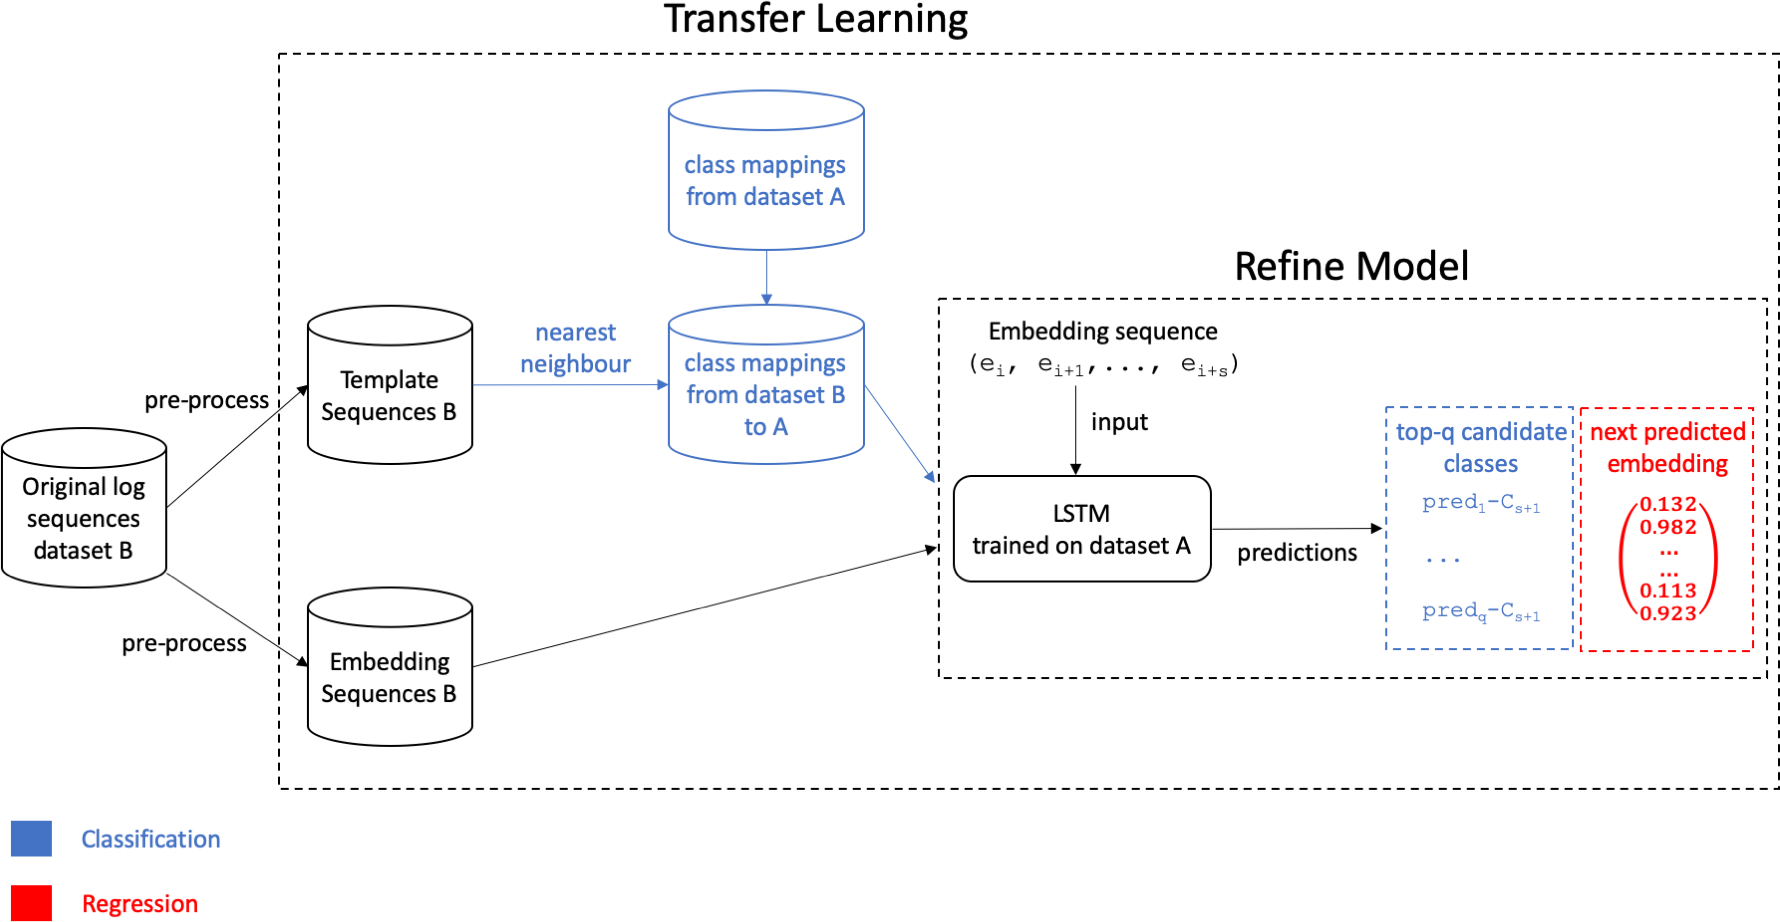
\includegraphics[width=16cm]{transfer-learning.png}
	\caption{Transfer Learning System}
	\label{fig:transfer_learning_system}
\end{figure}

\subsection{Classification \label{sec:transfer_classification}}
For the classification approach, the model is first trained as depicted in the pre-processing and training part of figure \ref{fig:overall_system} on a dataset A. Then, in order to re-use the trained model, several preliminary steps are executed. First, every log event of training dataset B is mapped to the nearest neighbour of dataset A, i.e. the word embedding with the shortest cosine distance, and gets assigned the same class. This is the same procedure as described in \ref{sec:classification} and depicted in \ref{fig:label_mapping}, with the only difference that there does not exist a threshold for assigning a class. Every log event will get a class assigned. Then, few-shot training on dataset B will be executed, in order to slightly adjust the model to the new dataset B. As a final step, with the adjusted model on training dataset B, the prediction phase on a test dataset B, exactly as described in \ref{sec:classification} can be executed.

\subsection{Regression \label{sec:transfer_regression}}
For transfer learning using the regression-based approach, no further adaptations are required - the model is trained on a given train dataset A, followed by few-shot training on a train dataset B. The model is then ready to make predictions on anomalies on a test dataset B using the approach described in \ref{sec:regression}.



\begin{figure}[htb]
  \centering
  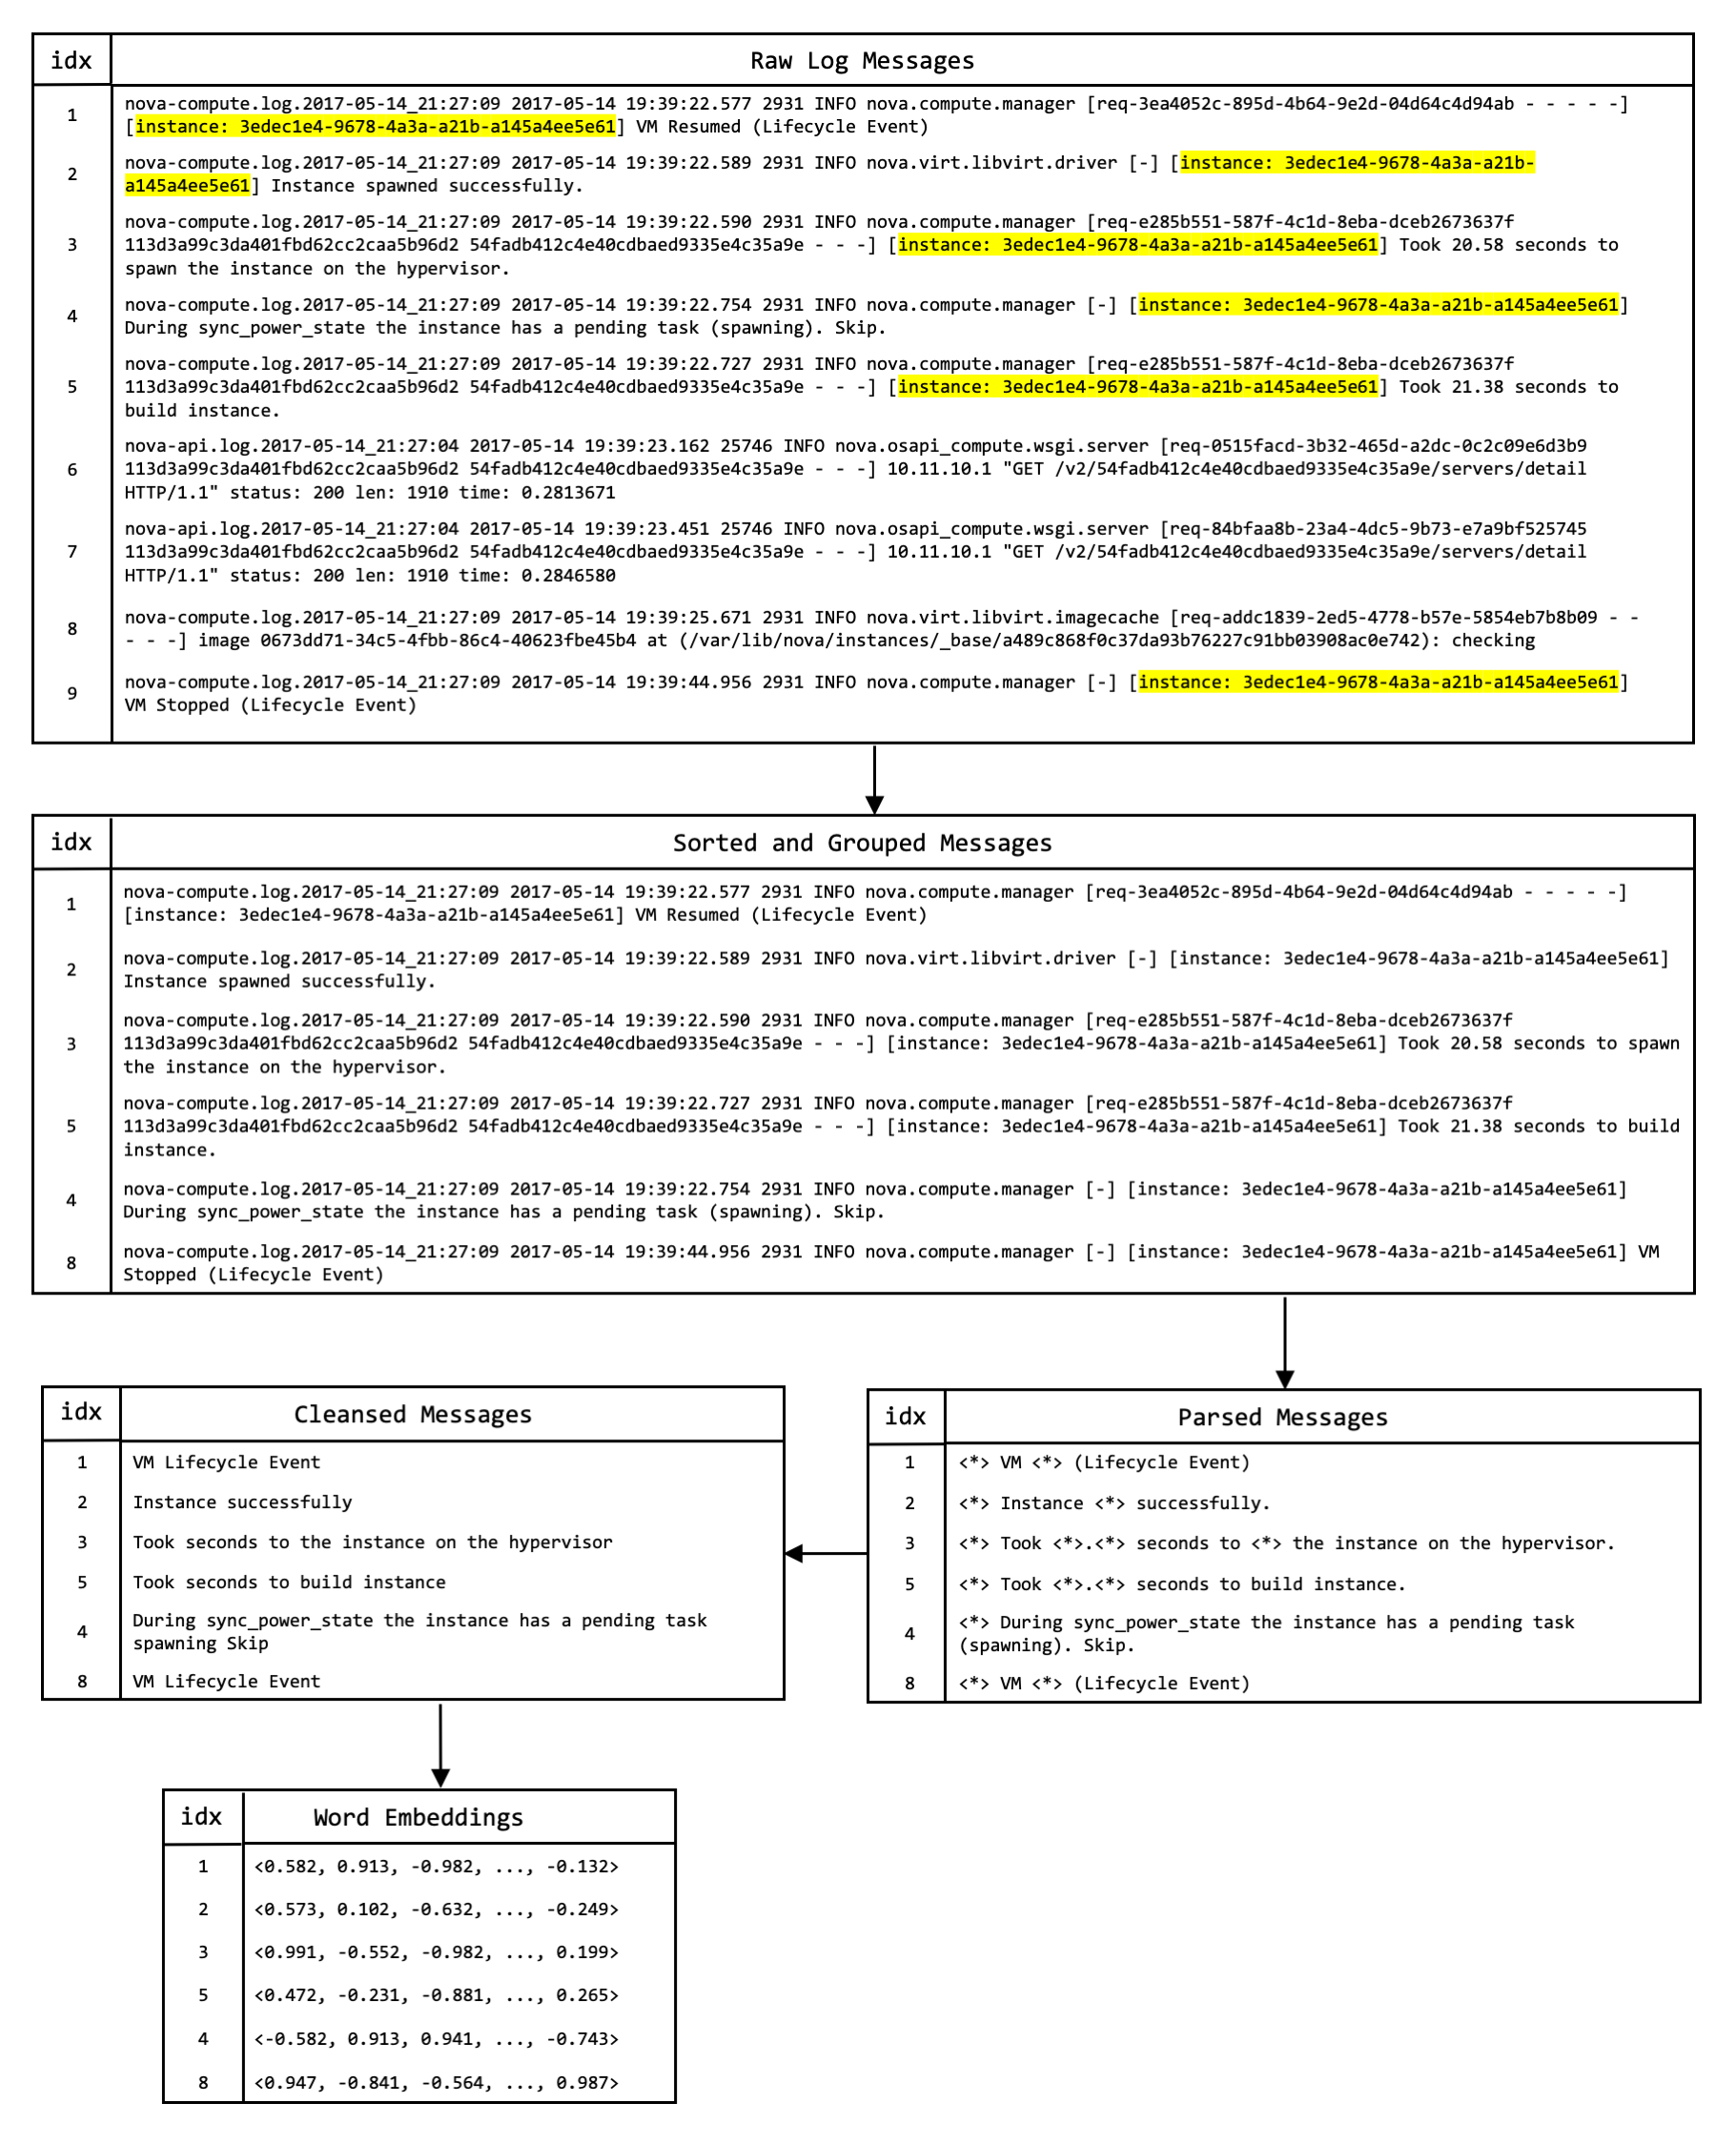
\includegraphics[width=14cm]{parsing_full.png}\\
  \caption{One full iteration of the pre-processing pipeline.}
  \label{fig:full_preprocessing_pipeline}
\end{figure}


\section{Possible Improvements and Extendibility\label{sec:improvements}}
In this section, possible improvements for the model are identified. 

In order to have more ways of evaluating different language models, next to the regression and multi-classification approach, a binary classification approach can be implemented.

To make the LSTM model more robust to alterations in a dataset, the attention mechanism, as described by Vaswani et al. \cite{vaswani2017attention} could be adopted.

The word embeddings are taken from the used language models as they are. Finetuning on the log corpora is only conducted using the default tasks that have been used to train the language model on extremely large corpora. The corpora on log data are likely to be too small. Even though most log events are sentences in English, they use very reduced idioms. A deeper investigation on how to train the language model specifically on the task of anomaly detection could potentially be useful in order to obtain better results.





